%% This is an example first chapter.  You should put chapter/appendix that you
%% write into a separate file, and add a line \include{yourfilename} to
%% main.tex, where `yourfilename.tex' is the name of the chapter/appendix file.
%% You can process specific files by typing their names in at the 
%% \files=
%% prompt when you run the file main.tex through LaTeX.

\chapter{Evaluations}\label{Chap:Evaluations}

This chapter presents evaluation metrics from the three case studies of the WebAuthn firewall. They put in concrete terms all of the advantages of the WebAuthn firewall discussed throughout this thesis. The principal evaluation critera focus on simplicity, organization, ease-of-use and performance overhead of the firewall.

\section{WebAuthn Firewall Configuration Metrics}

Each of the three case studies has its associated WebAuthn firewall configuration file. The number of lines of code of this file is a proxy measurement to evaluate the complexity and ease-of-use of the firewall. 

\subsection{Overall Complexity}

The total configuration file size evaluates the overall complexity of configuring the firewall. Table~\ref{Table:EvaluationOverallComplexity} lists the contents of a configuration file, sub-divided into four categories:

\begin{itemize}[nosep]

\item Configuration parameters as discussed in Section~\ref{Sec:ConfigurationParameters}

\item Context retrieval functions as discussed in Section~\ref{Sec:ContextRetrieval}

\item Domain specific language and custom route handlers as discussed in Sections~\ref{Sec:DomainSpecificLanguage} and~\ref{Sec:CustomHandlers}

\item Miscellaneous code such as extraneous syntax and boilerplate code

\end{itemize}

The file sizes and the respective four-way breakdown illustrate the overall and itemized complexity of using the firewall.
 
\begin{table}[h]
\centering

\begin{tabular}{ m{4.5cm} m{6cm}  } 
 \hline
 Case Study & Configuration File Lines of Code \\ 
 \hline \hline

 Conduit & 245 \\ \hline

 \quad Config Parameters & \quad 17 \\ \hline

 \quad Context Retrieval & \quad 117 \\ \hline

 \quad Route Handlers & \quad 49 \\ \hline

 \quad Miscellaneous & \quad 62 \\ \hline \hline

 Calypso & 253 \\ \hline

 \quad Config Parameters & \quad 22 \\ \hline

 \quad Context Retrieval & \quad 92 \\ \hline

 \quad Route Handlers & \quad 81 \\ \hline

 \quad Miscellaneous & \quad 58 \\ \hline \hline

 Gogs & 257 \\ \hline

 \quad Config Parameters & \quad 22 \\ \hline

 \quad Context Retrieval & \quad 51 \\ \hline

 \quad Route Handlers & \quad 126 \\ \hline

 \quad Miscellaneous & \quad 58 \\ \hline

\end{tabular}
\caption{A breakdown of the configuration file size for each case study. Each total is broken down into four categories with their respective lines of code contributions.}
\label{Table:EvaluationOverallComplexity}

\end{table}

The firewall configuration file is the sole source of customization that dictates how the firewall interacts with a specific web service. Both Calypso and Gogs are production web services. Considering that they are secured by the WebAuthn firewall within approximately 250 lines of code, this supports the claimed advantages of the firewall's simplicity and organization. 

\subsection{Incremental Complexity to Secure a Route}

The configuration parameters, context retrieval and miscellaneous code are more or less fixed costs to the configuration file's complexity. Only the route handlers scales with the size of the service being secured. Conduit being the smallest and simplest web service has the smallest route handler cost. Gogs, on the opposite end of the spectrum, naturally has the largest cost. Since most routes may be secured using the domain specific language, the increase in route handler complexity increases slowly.

Figure~\ref{Fig:IncrementalComplexity} plots the frequencies of lines of code needed to secure a new route among all three case studies. The bar chart can be partitioned into two clear clusters at approximately the 20 lines of code per route handler boundary. The bars on the left side with fewer than 20 lines correspond to uses of the domain specific language. The handlers greater than 20 lines of code are solely the custom handlers. It is natural to expect this divide since the custom handlers by nature perform more involved processing of a request than the DSL handlers and thus use more lines of code.

%% 
%% \iffalse
%%  where the lower end of lines of code per route handler, the bars on the left who represent routes with less than approximately 20 lines of code, correspond to uses of the domain specific language. 
%% \fi
%% 

\begin{figure}[h]
  \centering
  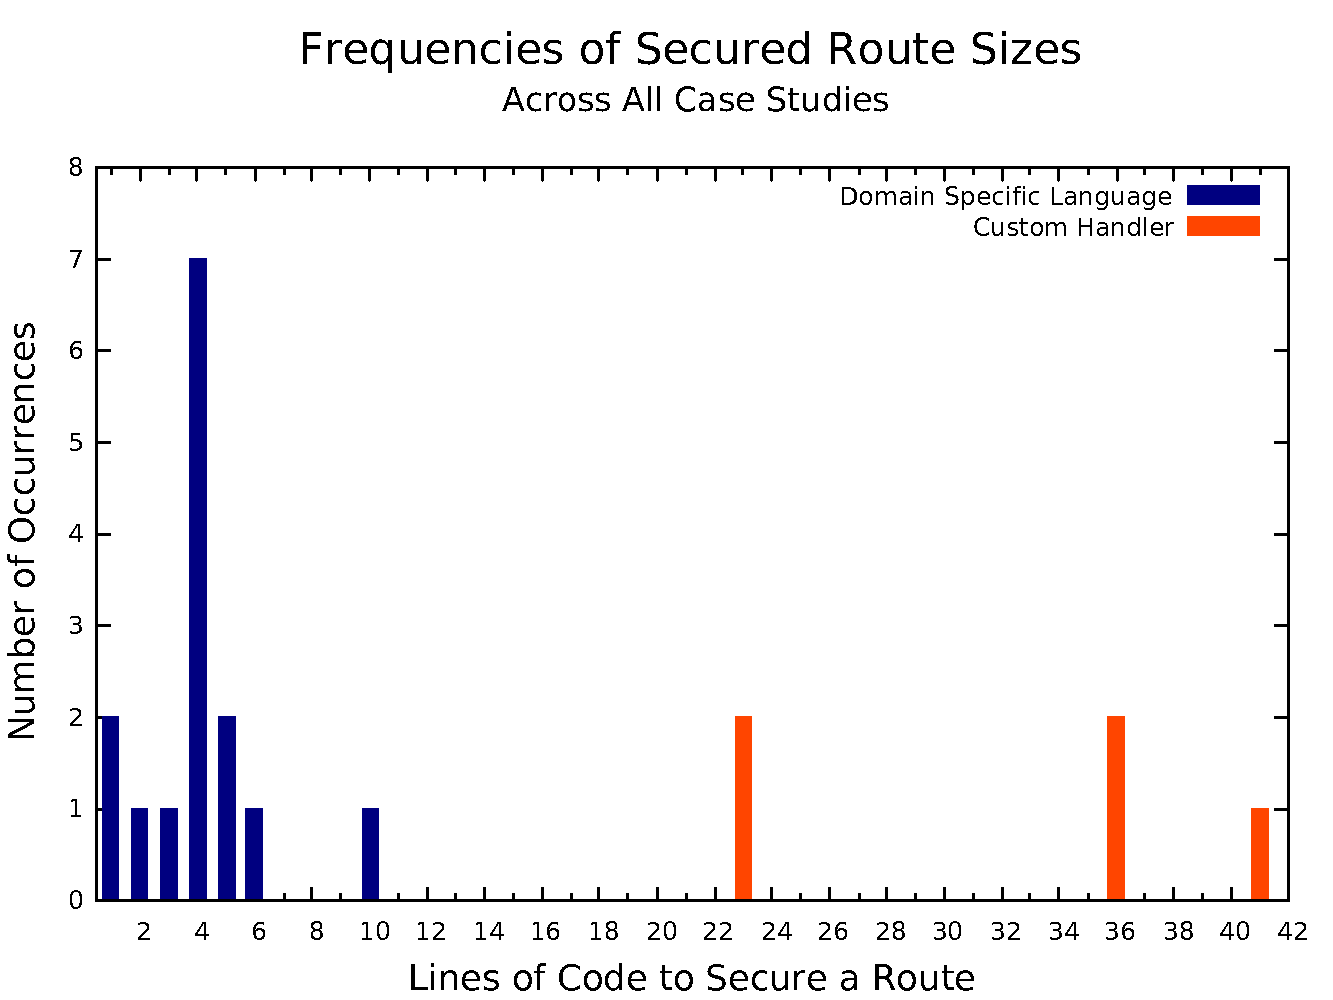
\includegraphics[width=14cm]{./plots/linesofcode}
  \caption{The frequencies of lines of code to secure a route with transaction authentication. The majority of the routes can be secured in 10 lines or less.}
  \label{Fig:IncrementalComplexity}
\end{figure}

This chart also evidently demonstrates that most of the routes may be secured using only the domain specific language. Of all 20 routes secured among all three case studies, only 5 required a custom handler. This means that 75\% of the routes could be captured by the domain specific language. The average domain specific program to secure a route is 4 lines of code, and the average custom handler is 32 lines of code. The total weighted average to secure a route is 11 lines of code.

%% 
%% \iffalse
%%  the domain specific language excises all of the boilerplate code wheras not handled directly in the custom handlers

%% , and they are secured using

%% The size of this configuration file and how much

%% A source of complexity when using the webauthn firewall is its configuraiton. These evaluation metrics demonstate that the firewall is 

%% In order to use the webauthn firewall on a web service, it must be configured. 

%% The total size, number of changes and 

%% Simplicity and organization

%%  are the main evaluation critera.
%% the benefits of using the firewall to integrate webauthn into a web service. 
%% \fi
%% 

\section{Frontend Modifications}

The frontend of a web service must be modified slightly when integrating WebAuthn, regardless of whether the WebAuthn firewall is in use or not. The frontend issuing the WebAuthn operation must adhere to the protocol specification life cycle as described in Chapter~\ref{Chap:WebauthnTransactionAuthentication}. Table~\ref{Table:EvaluationsFrontendModifications} lists the total number of code changes for each frontend of the case studies. For every case, the number of changes all exceed the sizes of the WebAuthn firewall configuration files.

\begin{table}[h]
\centering

\begin{tabular}{ m{4.5cm} m{6cm}  } 
 \hline
 Case Study & Frontend Lines of Code Changes \\ 
 \hline \hline

 Conduit & 289 \\ \hline

 Calypso & 402 \\ \hline

 Gogs & 570 \\ \hline

\end{tabular}
\caption{The number of code changes performed on each frontend of the case studies in order to support WebAuthn transaction authentication.}
\label{Table:EvaluationsFrontendModifications}
\end{table}

%% TODO: Not only gogs, but the overall average?
These code changes are not complex, but rather simple and monotonous. There is boilerplate code delegated to a JavaScript library. The nature of protecting an operation with WebAuthn on the frontend involves making a few library calls, error handling and piecing together the authentication message from the HTML data present. For example, each Gogs operation secured by WebAuthn involves on average 54 lines of code changes to the frontend. 

%% 
%% \iffalse
%% This includes the code to correctly format and encode data fields.

%% The boilerplate code is offloaded to a JavaScript library, but the library calls as well as piecing together the authentication message make up those changes.

%% \fi
%% 

\section{Backend Modifications}\label{Sec:BackendModifications}

A significant advantage to using the WebAuthn firewall over integrating WebAuthn intrusively into a web service is the lack of modifications needed to the backend. Table~\ref{Table:EvaluationsBackendModifications} demonstrates this fact --- using the WebAuthn firewall is minimally invasive to the backend.

\begin{table}[h]
\centering

\begin{tabular}{ m{4.5cm} m{6cm}  } 
 \hline
 Case Study & Backend Lines of Code Changes \\ 
 \hline \hline

 Conduit & 0 \\ \hline

 Calypso & 0 \\ \hline

 Gogs & 169 \\ \hline

\end{tabular}
\caption{The number of code changes performed on each backend of the case studies in order to support the WebAuthn firewall.}
\label{Table:EvaluationsBackendModifications}
\end{table}

The RESTful case studies, Conduit and Calypso, require no backend modifications. The Gogs case study, which is server-side rendered, only needs modifications to supply context. 

Before the WebAuthn firewall became a mature idea, Gogs was partly WebAuthn secured intrusively. The intrusive Gogs case study protects 5 routes whereas the WebAuthn firewall study of Gogs covers 11 routes. Nevertheless, even with fewer routes protected, the invasive nature of securing Gogs is unmistakable. Table~\ref{Table:EvaluationsComplexityDiffIntrusiveFirewall} backs this claim up plainly. The intrusive Gogs implementation is significantly more complex and more spread throughout Gogs than the WebAuthn firewall approach.

\begin{table}[h]
\centering

\begin{tabular}{ m{5cm} m{4.5cm} m{4.5cm}  } 
 \hline
 & Backend Lines Changed & Backend Files Modified \\ 
 \hline \hline

 Intrusive Gogs & 1293 & 18 \\ \hline

 WebAuthn Firewall Gogs & 169 & 5 \\ \hline


\end{tabular}
\caption{Comparing the complexity differences between intrusive and WebAuthn firewall integration.}
\label{Table:EvaluationsComplexityDiffIntrusiveFirewall}
\end{table}

Many of the additional lines of code for the intrusive WebAuthn integration of Gogs come from all of the plumbing code needed in to support and run WebAuthn. WebAuthn needs its own database table with entries to record registered users. The backend must support WebAuthn registration and login. It must also include the WebAuthn code that verifies transaction authentication events. All of these functionalities come with the WebAuthn firewall for free, which explains the dramatic reduction in backend complexity when using the firewall.

The firewall also dramatically reduces the amount of boilerplate code required to secure a new route. Gogs secured intrusively takes on average 87 lines of code per new route. The firewall has on average 11 lines per new route.

%% 
%% \iffalse
%% minimally invasive

%% Not all of the routes covered by the webauthn firewall case study of Gogs were done intrusively, but only the handful secured are enough to outline the minimal.
%% \fi
%% 

\section{Performance Overhead}

The WebAuthn firewall acts as a gatekeeper between the frontend and backend. It naturally adds some performance overhead to the whole system. This evaluation experiment measures the performance overhead under load to see how well it scales. 

The experiment's data are collected as follows. The hardware is a quad-core Intel i7-6600U CPU @ 2.60GHz laptop machine. Each trial initializes a given number of users. Then each user proceeds to sequentially send 300 POST requests to the ``Change Email'' route as quickly as possible, timing the latency of each request. The data point for the trial is the $95^{th}$ percentile of the running times tail. When there are many users sending requests simultaneously, there is contention among them which accounts for the increase in latency.

%% TODO: Make sure colors match up
Three different scenarios are tested and the results reported in Figure~\ref{Fig:PerformanceOverhead}. The blue line measures the request latencies for using the firewall on users that have WebAuthn enabled. The orange line measures the request latencies for the firewall on users without WebAuthn enabled. The difference between these two lines is the overhead of validating a WebAuthn transaction versus simply letting the request pass through. The yellow line measures the latencies of sending these requests to the backend directly.

\begin{figure}[h]
  \centering
  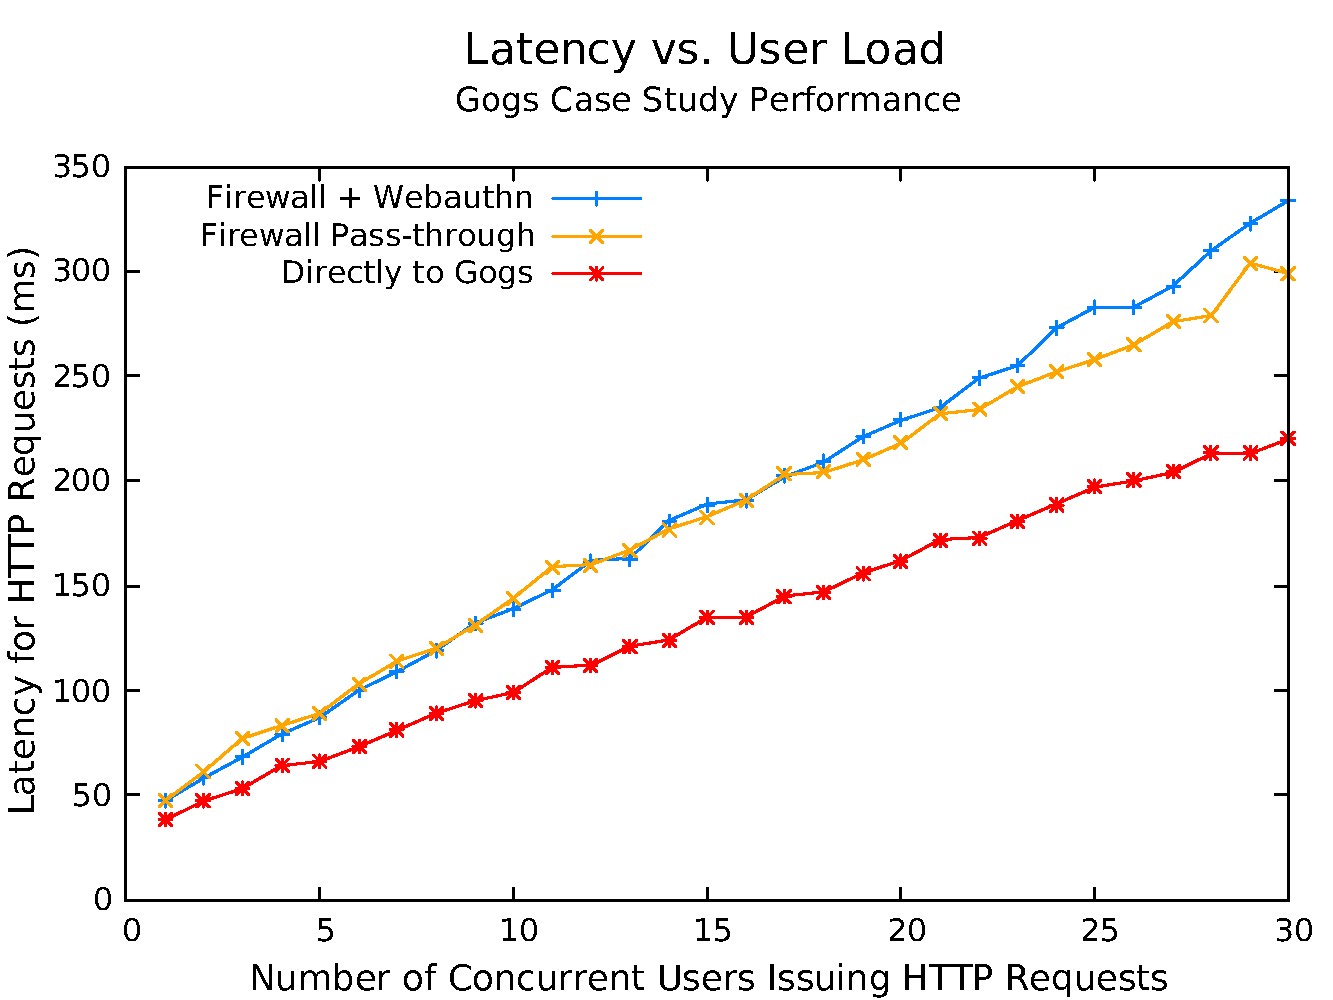
\includegraphics[width=13cm]{./plots/runtimes}
  \caption{The run times of three different Gogs setups under load. The x-axis are the number of users issuing requests concurrently, and the y-axis is the run time latency in milliseconds. The three experiments are: using the firewall with WebAuthn enabled, using the firewall with WebAuthn disabled, issuing requests directly to the Gogs server without WebAuthn transaction authentication. There is a latency penalty to using the WebAuthn firewall.}
  \label{Fig:PerformanceOverhead}
\end{figure}

As seen in Figure~\ref{Fig:PerformanceOverhead}, the blue and orange line remain tightly together meaning that there is little overhead from the actual validation of a WebAuthn transaction. Rather there is a significant gap between the direct connection and the firewall setup. This discrepancy arises from the implementation of the \lstinline{GetUserID} function of the Gogs firewall. The \lstinline{GetUserID} is a configurable function described in Section~\ref{Sec:ConfigurationParameters} which identifies the current user of a request received by the firewall. 

The firewall uses the current user information to determine for every incoming HTTP request whether that user has WebAuthn enabled and to verify the transaction accordingly if so. In Gogs, the user of a request is identified by a session ID, which only the backend can translate to a user ID. Therefore the \lstinline{GetUserID} for the Gogs firewall involves a HTTP GET request to the backend to retrieve the user ID. Therefore, every request that passes through the firewall invokes an additional HTTP request accounting for the substantial overhead when using the firewall. Under the 30 user load, the additional overhead of this \lstinline{GetUserID} operation added approximately 70 milliseconds to the overall latency.

The \lstinline{GetUserID} function is specific to the web service, and it is possible to design the software to avoid the additional HTTP call. The Conduit web service, for example, uses JSON Web Tokens (JWT) in order to identify the current user of an HTTP request. In this setup, the user ID is simply included in a signed JSON object with the request. The firewall can simply parse this data object and extract the identifier directly without any additional HTTP requests. Under such a setup, the latency discrepancy between the firewall and direct scenarios should diminish significantly.

%% 
%% \iffalse
%% There are three measurements

%% There naturally is a performance overhead suffered because of the .

%%   it naturally does add performance overhead.

%% Despite all of the advantages laid out by the webauthn firewall,
%% \fi
%% 
